%
% Main document
% ===========================================================================
% This is part of the document "Project documentation template".
% Authors: brd3, kaa1
%

%---------------------------------------------------------------------------
\documentclass[
	a4paper,					% paper format
	10pt,							% fontsize
	twoside,					% double-sided
	openright,				% begin new chapter on right side
	notitlepage,			% use no standard title page
	parskip=half,			% set paragraph skip to half of a line
]{scrreprt}					% KOMA-script report
%---------------------------------------------------------------------------

\raggedbottom
\KOMAoptions{cleardoublepage=plain}			% Add header and footer on blank pages


% Load Standard Packages:
%---------------------------------------------------------------------------
\usepackage[standard-baselineskips]{cmbright}

\usepackage[ngerman,english]{babel}										% english hyphenation
%\usepackage[latin1]{inputenc}  							% Unix/Linux - load extended character set (ISO 8859-1)
\usepackage[ansinew]{inputenc}  							% Windows - load extended character set (ISO 8859-1)
\usepackage[T1]{fontenc}											% hyphenation of words with �,� and �
\usepackage{textcomp}													% additional symbols
\usepackage{ae}																% better resolution of Type1-Fonts 
\usepackage{fancyhdr}													% simple manipulation of header and footer 
\usepackage{etoolbox}													% color manipulation of header and footer
\usepackage{graphicx}                      		% integration of images
\usepackage{float}														% floating objects
\usepackage{caption}													% for captions of figures and tables
\usepackage{booktabs}													% package for nicer tables
\usepackage{tocvsec2}													% provides means of controlling the sectional numbering
%---------------------------------------------------------------------------

% Load Math Packages
%---------------------------------------------------------------------------
\usepackage{amsmath}                    	   	% various features to facilitate writing math formulas
\usepackage{amsthm}                       	 	% enhanced version of latex's newtheorem
\usepackage{amsfonts}                      		% set of miscellaneous TeX fonts that augment the standard CM
\usepackage{amssymb}													% mathematical special characters
\usepackage{exscale}													% mathematical size corresponds to textsize
%---------------------------------------------------------------------------

% Package to facilitate placement of boxes at absolute positions
%---------------------------------------------------------------------------
\usepackage[absolute]{textpos}
\setlength{\TPHorizModule}{1mm}
\setlength{\TPVertModule}{1mm}
%---------------------------------------------------------------------------					
			
% Definition of Colors
%---------------------------------------------------------------------------
\RequirePackage{color}                          % Color (not xcolor!)
\definecolor{linkblue}{rgb}{0,0,0.8}            % Standard
\definecolor{darkblue}{rgb}{0,0.08,0.45}        % Dark blue
\definecolor{bfhgrey}{rgb}{0.41,0.49,0.57}      % BFH grey
%\definecolor{linkcolor}{rgb}{0,0,0.8}     			% Blue for the web- and cd-version!
\definecolor{linkcolor}{rgb}{0,0,0}        			% Black for the print-version!
%---------------------------------------------------------------------------

% Hyperref Package (Create links in a pdf)
%---------------------------------------------------------------------------
\usepackage[
	pdftex,ngerman,bookmarks,plainpages=false,pdfpagelabels,
	backref = {false},										% No index backreference
	colorlinks = {true},                  % Color links in a PDF
	hypertexnames = {true},               % no failures "same page(i)"
	bookmarksopen = {true},               % opens the bar on the left side
	bookmarksopenlevel = {0},             % depth of opened bookmarks
	pdftitle = {Template f�r Bachelor Thesis},	   	% PDF-property
	pdfauthor = {brd3},        					  % PDF-property
	pdfsubject = {LaTeX Template},        % PDF-property
	linkcolor = {linkcolor},              % Color of Links
	citecolor = {linkcolor},              % Color of Cite-Links
	urlcolor = {linkcolor},               % Color of URLs
]{hyperref}
%---------------------------------------------------------------------------

% Set up page dimension
%---------------------------------------------------------------------------
\usepackage{geometry}
\geometry{
	a4paper,
	left=28mm,
	right=15mm,
	top=30mm,
	headheight=20mm,
	headsep=10mm,
	textheight=242mm,
	footskip=15mm
}
%---------------------------------------------------------------------------

% Makeindex Package
%---------------------------------------------------------------------------
\usepackage{makeidx}                         		% To produce index
\makeindex                                    	% Index-Initialisation
%---------------------------------------------------------------------------

% Glossary Package
%---------------------------------------------------------------------------
% the glossaries package uses makeindex
% if you use TeXnicCenter do the following steps:
%  - Goto "Ausgabeprofile definieren" (ctrl + F7)
%  - Select the profile "LaTeX => PDF"
%  - Add in register "Nachbearbeitung" a new "Postprozessoren" point named Glossar
%  - Select makeindex.exe in the field "Anwendung" ( ..\MiKTeX x.x\miktex\bin\makeindex.exe )
%  - Add this [ -s "%tm.ist" -t "%tm.glg" -o "%tm.gls" "%tm.glo" ] in the field "Argumente"
%
% for futher informations go to http://ewus.de/tipp-1029.html
%---------------------------------------------------------------------------
\usepackage[nonumberlist]{glossaries}
\makeglossaries

\newglossaryentry{BibTeX}{name={BibTeX},description={Program for the creation of 	bibliographical references and directories in \TeX or \LaTeX documents}}
\newglossaryentry{Index}{name={Index},description={Index with keywords from text}}



%---------------------------------------------------------------------------

% Intro:
%---------------------------------------------------------------------------
\begin{document}                              	% Start Document
\settocdepth{section}														% Set depth of toc
\pagenumbering{roman}														
%---------------------------------------------------------------------------

\providecommand{\heading}{Remote Signing Service}		%  Insert Title of Thesis here					% Titel der Arbeit aus Datei titel.tex lesen
\providecommand{\versionnumber}{13.3.7}			%  Hier die aktuelle Versionsnummer eingeben
\providecommand{\versiondate}{\today}		%  Hier das Datum der aktuellen Version eingeben				% Versionsnummer und -datum aus Datei version.tex lesen

% Set up header and footer
%---------------------------------------------------------------------------
\makeatletter
\patchcmd{\@fancyhead}{\rlap}{\color{bfhgrey}\rlap}{}{}		% new color of header
\patchcmd{\@fancyfoot}{\rlap}{\color{bfhgrey}\rlap}{}{}		% new color of footer
\makeatother

\fancyhf{}																		% clean all fields
\fancypagestyle{plain}{												% new definition of plain style	
	\fancyfoot[OR,EL]{\footnotesize \thepage} 	% footer right part --> page number
	\fancyfoot[OL,ER]{\footnotesize \heading, Version \versionnumber, \versiondate}	% footer even page left part 
}

\renewcommand{\chaptermark}[1]{\markboth{\thechapter.  #1}{}}
\renewcommand{\headrulewidth}{0pt}				% no header stripline
\renewcommand{\footrulewidth}{0pt} 				% no bottom stripline

\pagestyle{plain}
%---------------------------------------------------------------------------


% Title Page and Abstract
%---------------------------------------------------------------------------
%%
% Project documentation template
% ===========================================================================
% This is part of the document "Project documentation template".
% Authors: brd3, kaa1
%

\begin{titlepage}


% BFH-Logo absolute placed at (28,12) on A4 and picture (16:9 or 15cm x 8.5cm)
% Actually not a realy satisfactory solution but working.
%---------------------------------------------------------------------------
\setlength{\unitlength}{1mm}
\begin{textblock}{20}[0,0](28,12)
	
\includegraphics[scale=1.0]{images/BFH_Logo_B.png}
\end{textblock}

% Institution / titel / subtitel / authors / experts:
%---------------------------------------------------------------------------
\begin{flushleft}

\vspace*{21mm}

\fontsize{26pt}{40pt}\selectfont 
\heading				\\							% Read heading from file leader/title.tex
\vspace{2mm}

\fontsize{16pt}{24pt}\selectfont\vspace{0.3em}
Accessible Electronic Signatures for Everybody 			\\				% Insert subheading
\vspace{5mm}

\fontsize{10pt}{12pt}\selectfont
\textbf{Bachelor Thesis by Gabor Tanz and Patrick Hirt} \\		% Insert text
\vspace{7mm}

% Abstract (eingeben):
%---------------------------------------------------------------------------
\begin{textblock}{150}(28,100)
\fontsize{10pt}{12pt}\selectfont
    TODO abstract TODO
\end{textblock}

\begin{textblock}{150}(28,225)
\fontsize{10pt}{17pt}\selectfont
\begin{tabbing}
xxxxxxxxxxxxxxx\=xxxxxxxxxxxxxxxxxxxxxxxxxxxxxxxxxxxxxxxxxxxxxxx \kill
Degree course:	\> [z.B. Electrical and Communication Engineering]	\\		% insert name of degree course
Authors:		\> [Test Peter, M\"uster R\"os\"a]		\\					% insert names
Tutor:	\> [Dr.~Xxxx Xxxx, Dr.~Yyyy Yyyy]		\\							% insert names
Constituent:	\> [Wwwww AG]					\\							% insert names
Experts:		\> [Dr.~Zzzz Zzzz]				\\							% insert names
Date:			\> \versiondate					\\							% read from file leader/version.tex
\end{tabbing}

\end{textblock}
\end{flushleft}

\begin{textblock}{150}(28,280)
\noindent 
\color{bfhgrey}\fontsize{9pt}{10pt}\selectfont
Berner Fachhochschule | Haute \'ecole sp\'ecialis\'ee bernoise | Bern University of Applied Sciences
\color{black}\selectfont
\end{textblock}


\end{titlepage}

%
% ===========================================================================
% EOF
%
		% activate for frontpage without picture
%
% Project documentation template
% ===========================================================================
% This is part of the document "Project documentation template".
% Authors: brd3, kaa1
%

\begin{titlepage}


% BFH-Logo absolute placed at (28,12) on A4 and picture (16:9 or 15cm x 8.5cm)
% Actually not a realy satisfactory solution but working.
%---------------------------------------------------------------------------
\setlength{\unitlength}{1mm}
\begin{textblock}{20}[0,0](28,12)
	
\includegraphics[scale=1.0]{images/BFH_Logo_B.png}
\end{textblock}

\begin{textblock}{154}(28,48)
	\begin{picture}(150,2)
		\put(0,0){\color{bfhgrey}\rule{150mm}{2mm}}
	\end{picture}
\end{textblock}

\begin{textblock}{154}[0,0](28,50)
	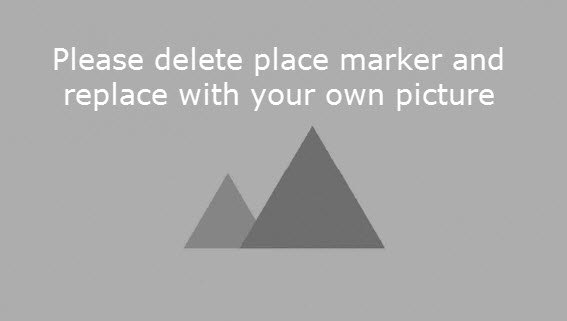
\includegraphics[scale=1.0]{images/placemarker.jpg}			% define cover picture
\end{textblock}

\begin{textblock}{154}(28,135)
	\begin{picture}(150,2)
		\put(0,0){\color{bfhgrey}\rule{150mm}{2mm}}
	\end{picture}
\end{textblock}
\color{black}

% Institution / titel / subtitel / authors / experts:
%---------------------------------------------------------------------------
\begin{flushleft}

\vspace*{115mm}

\fontsize{26pt}{28pt}\selectfont 
\heading				\\							% Read heading from file leader/title.tex
\vspace{2mm}

\fontsize{16pt}{20pt}\selectfont\vspace{0.3em}
Place your subheading here 			\\				% Insert subheading
\vspace{5mm}

\fontsize{10pt}{12pt}\selectfont
\textbf{Description of thesis (semester- / Bachelor thesis / etc.)} \\		% Insert text
\vspace{3mm}

% Abstract (eingeben):
%---------------------------------------------------------------------------
\begin{textblock}{150}(28,190)
\fontsize{10pt}{12pt}\selectfont
[Insert short text (abstract) if desired] \\ 
This document serves as a template for the compilation of reports according to the guidelines of the BFH. The template is written in LATEX and supports the automatic writing of various directories, references, indexing and glossaries. This small text is a summary of this document with a length of 4 to max. 8 lines. \\ 
The cover picture may be turned on or off in the lines 157/158 of the file template.tex.
\end{textblock}

\begin{textblock}{150}(28,225)
\fontsize{10pt}{17pt}\selectfont
\begin{tabbing}
xxxxxxxxxxxxxxx\=xxxxxxxxxxxxxxxxxxxxxxxxxxxxxxxxxxxxxxxxxxxxxxx \kill
Degree course:	\> [z.B. Electrical and Communication Engineering]	\\		% insert name of degree course
Authors:		\> [Test Peter, M\"uster R\"os\"a]		\\					% insert names
Tutor:	\> [Dr.~Xxxx Xxxx, Dr.~Yyyy Yyyy]		\\							% insert names
Constituent:	\> [Wwwww AG]					\\							% insert names
Experts:		\> [Dr.~Zzzz Zzzz]				\\							% insert names
Date:			\> \versiondate					\\							% read from file leader/version.tex
\end{tabbing}

\end{textblock}
\end{flushleft}

\begin{textblock}{150}(28,280)
\noindent 
\color{bfhgrey}\fontsize{9pt}{10pt}\selectfont
Berner Fachhochschule | Haute \'ecole sp\'ecialis\'ee bernoise | Bern University of Applied Sciences
\color{black}\selectfont
\end{textblock}


\end{titlepage}

%
% ===========================================================================
% EOF
%
		% activate for frontpage with picture
% Control of versions :
% -----------------------------------------------

\begin{textblock}{180}(15,150)
\color{black}
\begin{huge}
Versions
\end{huge}
\vspace{10mm}

\fontsize{10pt}{18pt}\selectfont
\begin{tabbing}
xxxxxxxxxxx\=xxxxxxxxxxxxxxx\=xxxxxxxxxxxxxx\=xxxxxxxxxxxxxxxxxxxxxxxxxxxxxxxxxxxxxxxxxxxxxxx \kill
Version	\> Date	\> Status			\> Remarks		\\
0.1	\> 01.08.2013	\> Draft		\> Lorem ipsum dolor sit amet	\\	
0.2	\> 21.08.2013	\> Draft		\> Phasellus scelerisque	\\ 
0.3	\> 02.09.2013	\> Draft		\> Donec eget aliquam urna. Lorem ipsum dolor sit amet	\\ 
1.0	\> 26.01.2014	\> Final		\> Lorem ipsum dolor sit ametPhasellus scelerisque, leo sed iaculis ornare 	\\ 
1.1	\> 31.01.2014	\> Correction	\> Layout changed	\\
1.2	\> 07.02.2014	\> Addition		\> Chapter 1.1 extended	\\
\end{tabbing}

\end{textblock}

\cleardoubleemptypage
\setcounter{page}{1}
\cleardoublepage
\phantomsection 
\addcontentsline{toc}{chapter}{Management Summary}
\chapter*{Management Summary}
\label{chap:managementSummary}

Lorem ipsum dolor sit amet, consectetur adipiscing elit. Phasellus scelerisque, leo sed iaculis ornare, mi leo semper urna, ac elementum libero est at risus. Donec eget aliquam urna. Lorem ipsum dolor sit amet, consectetur adipiscing elit. Nunc fermentum nunc sollicitudin leo porttitor volutpat. Duis ac enim lectus, quis malesuada lectus. Aenean vestibulum suscipit justo, in suscipit augue venenatis a. Donec interdum nibh ligula. Aliquam vitae dui a odio cursus interdum quis vitae mi. Phasellus ornare tortor fringilla velit accumsan quis tincidunt magna eleifend. Praesent nisl nibh, cursus in mattis ac, ultrices ac nulla. Nulla ante urna, aliquet eu tempus ut, feugiat id nisl. Nunc sit amet mauris vitae turpis scelerisque mattis et sed metus. Aliquam interdum congue odio, sed semper elit ullamcorper vitae. Morbi orci elit, feugiat vel hendrerit nec, sollicitudin non massa. Quisque lacus metus, vulputate id ullamcorper id, consequat eget orci \nocite{kopka:band1} \nocite{Marti06}. 

\cleardoubleemptypage
%---------------------------------------------------------------------------

% Table of contents
%---------------------------------------------------------------------------
\tableofcontents
\cleardoublepage
%---------------------------------------------------------------------------

% Main part:
%---------------------------------------------------------------------------
\pagenumbering{arabic}

\chapter{Introduction}
\label{sec:introduction}

Today, we use a number of computing devices interchangeably on a daily basis: a desktop workstation at the office,
a laptop computer on the move, a tablet in the living room and of course, always by our side, the smartphone.
In an increasingly cloudified and mobile world our expectation is to be able to do our work all the same,
regardless of the computing device we use, or where we are.

We start editing a text document in Google Docs on our desktop workstation at the office,
work on it a bit more on our laptop while travelling by train,
and proofread it later on the smartphone.
This device- and location-independent way of working has become the standard in recent years,
and users have started to expect it from their IT devices.

It's difficult to meet this expectation with the way electronic signatures are usually created today,
using certificates stored on on smartcards,
plugged into a laptop,
using a specialised card reader and accompanying software.
It's annoying and inconvenient having to carry around cables and adaptors, and a lot can go wrong:
a random operating system update breaking driver compatibility with the card reader, for example,
leaving us dead in the water.
If we want to make this easier on the user and to drive usage of electronic signatures and even make them mainstream,
we have to do better.

At the root of this inconvenience is the requirement that the user keep their private key physically with them,
stored in a manner making it difficult for anyone to steal it: on a smartcard.
Any IT professional knows full well this demand isn't made from users in order to annoy them but because it is
- more or less - the only practical \textit{and} secure way to have users store their private key.

So-called Remote Signing Services aim to eliminate the need for people to carry their private key with them,
and to locally create signatures,
in the hope for improved ease of use, and eventually, greater adoption of digitally signing documents.
However, allowing someone (the signing service, in this case) to be able to sign documents in place of the user introduces a number of serious security and confidentiality problems.


In this thesis, we analyse and address these problems,
and we implement the proposed solutions in a fully functional Remote Signing Service,
thereby showing that they work in the real world and not just on paper.

We will allow people to create electronic signatures,
no matter where they are, or what device they're using,
in a secure manner.
Building on our previous work of Projekt 2~\cite{projekt2}, we show how it is possible to securely integrate \gls{OIDC} authentication with remote digital signatures.
We expand upon this previous work and show how it is possible to have a remote signing service with the capability of signing on the users' behalf without the need for completely trusting that service.
Furthermore, we compare our solutions to those proposed by an industrial consortium led by Adobe Inc.,
and we show in which ways we believe our approach to be superior.


\chapter{Instructions}
\label{chap:instructions}

The following table shows some of the most important packages\index{packages} used in the \LaTeX{} template.

\begin{table}[H]
	\centering
		\begin{tabular}{p{0.13\textwidth} p{0.75\textwidth}} \toprule
			\textbf{Package} & \textbf{Function} \\ \midrule
			\texttt{cmbright}\index{cmbright} & sans serif font "Computer Modern Bright", which supports text encodings\index{text encodings} OT1, T1 and TS1, as well as the mathematical signs and AMS symbols \\ \midrule
			\texttt{ae} & provides better resolution fonts in PDF files \\ \midrule
			\texttt{fancyhdr}\index{fancyhdr} & easy adjustment of head- and foot lines \\ \midrule
			\texttt{graphicx}\index{graphicx} & integration of graphics in \LaTeX{} documents \\ \midrule
			\texttt{booktabs}\index{booktabs} & better presentation of tables \\ \midrule
			\texttt{textpos}\index{textpos} & simplified and absolute positioning of boxes on the page \\ \midrule
			\texttt{hyperref}\index{hyperref} & package to complie links into PDF files \\ \midrule
			\texttt{geometry}\index{geometry} & simplified and improved adaptation of the standard type area \\ \midrule
			\texttt{makeidx}\index{makeidx} & simple Index compilation (see section \ref{sec:instructions_index}) \\ \midrule
			\texttt{glossaries}\index{glossaries} & compilation of glossaries (see section \ref{sec:instructions_glossay}) \\ \bottomrule
		\end{tabular}
	\caption{Packages}
	\label{tab:packages}
\end{table}


\section{Subject Indices}
\label{sec:instructions_index}

\LaTeX{} is not able to create an \gls{Index}\index{Index} in the basic configuration. This can be created in \LaTeX{} with the \texttt{makeidx} package and the \texttt{makeindex}\index{makeindex} program. The following page contains a detailed explanation of how the package works, and its application:

\begin{center}
	\url{http://en.wikibooks.org/wiki/LaTeX/Indexing}
\end{center}

Roughly summarized the following points are needed for an index:

\begin{itemize}
	\item Embed the package \texttt{makeidx}.
	\item Initialize the compilation with the command \texttt{\textbackslash makeindex}.
	\item Continuously initializing words in the text with the command \texttt{\textbackslash index\{\}}.
	\item During the first passage of the document's compilation, the directory is created and definitions marked with \texttt{\textbackslash index\{\}} are stored in the \texttt{.idx} file.
	\item During the second passage the \texttt{.idx} file is sorted, formatted and stored as \texttt{.ind} file whereas \LaTeX{} then inserts the \texttt{.ind} file into the document.
\end{itemize}

\section{Glossay}
\label{sec:instructions_glossay}

A glossary\index{glossary} can also be created in \LaTeX{} with the \texttt{makeindex} program and the \texttt{glossaries} package. The following list shows the procedure to generate a glossary:

\begin{itemize}
	\item Integration of the package \texttt{glossaries}.
	\item If necessary, a personal database may be created including glossary entries. This template works with such a database, which is stored in the \texttt{database}folder. Entries from the database are only written in the directory if the word in the text is actually stated.
	\item With the \texttt{\textbackslash makeglossaries} command a new compilation is initialized.
	\item New entries can be created with the command \\ \texttt{\textbackslash newglossaryentry\{<SHORTCUT>\}\{name=\{<NAME>\},description=\{<DESCRIPTION>\}\}}.
	\item In the text continuously referencing words with the command \texttt{\textbackslash gls\{<SHORTCUT>\}}.
	\item Similar to the compilation of the index, the directory is only embedded into the document  during the second passage.
\end{itemize}

In order to work accurately, the glossary must be compiled with \texttt{makeindex} after post-editing the document. For this the following code in the command line is to be executed:

\begin{center}
	\texttt{makeindex -s template.ist -t template.glg -o template.gls template.glo}
\end{center}

With most \LaTeX editors, this can be stated as a post-processing step. The following explanation is for the TeXnicCenter program. Under the menu "Build" > "Define Output Profile..." (short: alt + F7) in the "Postprocessor" register, the window shown in Figure \ref{fig:postprocessing} can be found. Then it is necessary to insert a new entry, when an application as well as an argument must be specified. The application can be found in the MiKTeX installation (\texttt{..\textbackslash MiKTeX X.X\textbackslash miktex\textbackslash bin\textbackslash makeindex.exe}). As an argument, the following line must be entered:

\begin{center}
	\texttt{-s \string"\%tm.ist\string" -t \string"\%tm.glg\string" -o \string"\%tm.gls\string" \string"\%tm.glo\string" }
\end{center}

\begin{figure}[H]
	\centering
		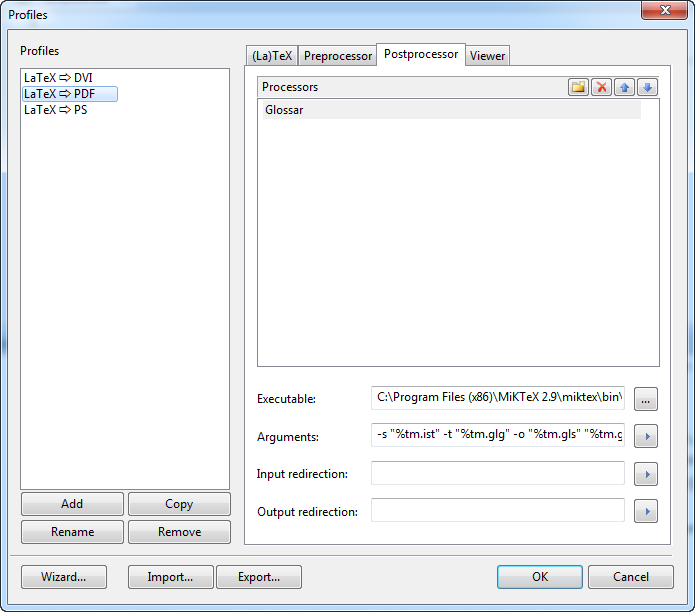
\includegraphics[scale=0.6]{images/profiles_glossar.png}
	\caption{Post-processing}
	\label{fig:postprocessing}
\end{figure}


\section{Bibliography}
\label{sec:instructions_bibliography}

To compile a bibliography\index{bibliography} one must resort to \gls{BibTeX}. The folder \texttt{database} includes a \texttt{.bib} file with various database entries. How the entries are to be compiled, can be taken from various sources of the Internet or books. The entries in the database will only be written to the directory of the document when the source is actually cited in the text.

Under the following addresses further explanations are found in order to compile the database and its use:

\begin{itemize}
	\item \url{http://en.wikipedia.org/wiki/BibTeX}
	\item \url{http://www.bibtex.org/}
\end{itemize}



\chapter{Test of type area}
\label{chap:typeareatest}

Far far away, behind the word mountains, far from the countries Vokalia and Consonantia, there live the blind texts. Separated they live in Bookmarksgrove right at the coast of the Semantics, a large language ocean. A small river named Duden flows by their place and supplies it with the necessary regelialia. It is a paradisematic country, in which roasted parts of sentences fly into your mouth. Even the all-powerful Pointing has no control about the blind texts it is an almost unorthographic life One day however a small line of blind text by the name of Lorem Ipsum decided to leave for the far World of Grammar. 

\section{The Big Oxmox}
\label{sec:typeareatest_ombox}

The Big Oxmox advised her not to do so, because there were thousands of bad Commas, wild Question Marks and devious Semikoli, but the Little Blind Text didn’t listen. She packed her seven versalia, put her initial into the belt and made herself on the way. When she reached the first hills of the Italic Mountains, she had a last view back on the skyline of her hometown Bookmarksgrove, the headline of Alphabet Village and the subline of her own road, the Line Lane. Pityful a rethoric question ran over her cheek, then she continued her way. On her way she met a copy.

\begin{equation}
	\mathcal{N}(x \mid \mathbold{\mu}, \mathbold{\Sigma}) = \frac{1}{(2\pi)^{D/2}} \frac{1}{|\mathbold{\Sigma}|^{(1/2)}} \exp \left( -\frac{1}{2}(x-\mathbold{\mu})^{T}\mathbold{\Sigma}^{-1}(x-\mathbold{\mu}) \right)
\end{equation}

The copy warned the Little Blind Text, that where it came from it would have been rewritten a thousand times and everything that was left from its origin would be the word "and" and the Little Blind Text should turn around and return to its own, safe country. But nothing the copy said could convince her and so it didn’t take long until a few insidious Copy Writers ambushed her, made her drunk with Longe and Parole and dragged her into their agency, where they abused her for their projects again and again. And if she hasn’t been rewritten, then they are still using her.

\section{Type dummy text}
\label{sec:typeareatest_typedummytext}

This is a typo dummy text. On it you can see if all the letters there are and how they look. Sometimes one uses words like Hamburgefonts, Rafgenduks or Handgloves to test fonts. Sometimes phrases that contain all letters of the alphabet - one calls these sets "pangrams".

Well known is this: The quick brown fox jumps over the lazy old dog. Often in type dummy texts also foreign-language sentence parts are installed (AVAIL\textsuperscript{\texttrademark} and Wefox\textsuperscript{\textregistered} are testing aussi la Kerning) to test the effect in other languages. In Latin, for example, almost every font looks good.

\subsection{Demonstrandum}
\label{subsec:satzspiegeltest_typoblindtext_demonstrandum}

Quod erat demonstrandum. Seit 1975 fehlen in den meisten Testtexten die Zahlen, weswegen nach TypoGb. 204 \S ab dem Jahr 2034 Zahlen in 86 der Texte zur Pflicht werden. Nichteinhaltung wird mit bis zu 245 \texteuro oder 368\$ bestraft. Genauso wichtig in sind mittlerweile auch \^A\c{c}c\`e\~nt\"e, die in neueren Schriften aber fast immer enthalten sind. Ein wichtiges aber schwierig zu integrierendes Feld sind OpenType-Funktionalit\"aten. Je nach Software und Voreinstellungen k\"onnen eingebaute Kapit\"alchen, Kerning oder Ligaturen (sehr pfiffig) nicht richtig dargestellt werden.

\subsubsection{Subsubsection}

This is a typo dummy text. On it you can see if all the letters there are and how they look. Sometimes one uses words like Hamburgefonts, Rafgenduks or Handgloves to test fonts. Sometimes phrases that contain all letters of the alphabet - one calls these sets "pangrams". 

\subsubsection{Subsubsection}

Well known is this: The quick brown fox jumps over the lazy old dog. Often in type dummy texts also foreign-language sentence parts are installed (AVAIL\textsuperscript{\texttrademark} and Wefox\textsuperscript{\textregistered} are testing aussi la Kerning) to test the effect in other languages. In Latin, for example, almost every font looks good. Quod erat demonstrandum.

\section{Webstandards}
\label{sec:satzspiegeltest_webstandards}

Everywhere the same old story. The layout is complete, the text is slow in coming. This layout is now not naked in space and small and empty occurs, I help out: the dummy text. Created exactly for this purpose, always in the shadow of my big brother "Lorem Ipsum", I look forward every time you read a few lines. Because esse est percipi - being is to be perceived.

And now because you already have the goodness to accompany me a few more sentences long, I would like to take this opportunity to serve you not only as a stopgap, but to point out something that is going to be perceived as deserved: Web viz. See Web standards are the rules that build on the websites. So there are rules for HTML, CSS, JavaScript or XML, words that you might have heard of your developers. These standards ensure that all parties the maximum benefit from a website.

\begin{figure}[H]
	\centering
		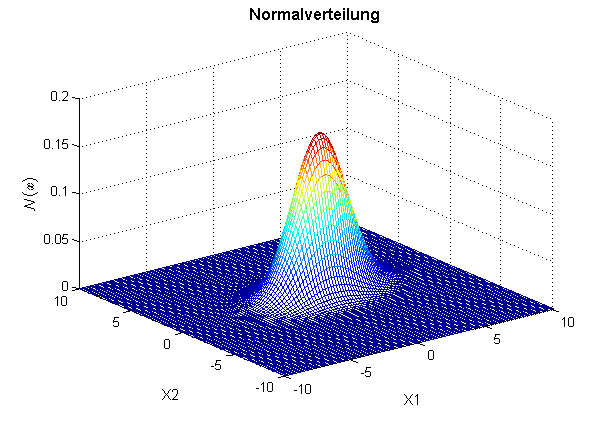
\includegraphics[scale=0.7]{images/multivariate_gauss.png}
	\caption{Normal distribution}
	\label{fig:normal_distribution}
\end{figure}

In contrast to previous websites we no longer need, for example, two different sites for the program Internet Explorer and another browser. It extends a page that - properly applied - both works on different browsers on the net, but just as good for printing or display on a cell phone is. Mind: A site for all formats. What a relief. Standards save time provide for the development costs and ensure that web pages can be easier to maintain later. Of course, only if everyone adheres to these standards.

\chapter{Conclusion / Results}
\label{chap:conclusions}

But I must explain to you how all this mistaken idea of denouncing pleasure and praising pain was born and I will give you a complete account of the system, and expound the actual teachings of the great explorer of the truth, the master-builder of human happiness. No one rejects, dislikes, or avoids pleasure itself, because it is pleasure, but because those who do not know how to pursue pleasure rationally encounter consequences that are extremely painful. Nor again is there anyone who loves or pursues or desires to obtain pain of itself, because it is pain, but because occasionally circumstances occur in which toil and pain can procure him some great pleasure. To take a trivial example, which of us ever undertakes laborious physical exercise, except to obtain some advantage from it? But who has any right to find fault with a man who chooses to enjoy a pleasure that has no annoying consequences, or one who avoids a pain that produces no resultant pleasure? On the other hand, we denounce with righteous indignation and dislike men who are so beguiled and demoralized by the charms of pleasure of the moment, so blinded by desire, that they cannot foresee the pain and trouble that are bound to ensue; and equal blame belongs to those who fail in their duty through weakness of will, which is the same as saying through shrinking from toil and pain. These cases are perfectly simple and easy to distinguish. In a free hour, when our power of choice is untrammelled and when nothing prevents our being able to do what we like best, every pleasure is to be welcomed and every pain avoided. But in certain circumstances and owing to the claims of duty or the obligations of business it will frequently occur that pleasures have to be repudiated and annoyances accepted. The wise man therefore always holds in these matters to this principle of selection: he rejects pleasures to secure other greater pleasures, or else he endures pains to avoid worse pains.

\newpage

But I must explain to you how all this mistaken idea of denouncing pleasure and praising pain was born and I will give you a complete account of the system, and expound the actual teachings of the great explorer of the truth, the master-builder of human happiness. No one rejects, dislikes, or avoids pleasure itself, because it is pleasure, but because those who do not know how to pursue pleasure rationally encounter consequences that are extremely painful. Nor again is there anyone who loves or pursues or desires to obtain pain of itself, because it is pain, but because occasionally circumstances occur in which toil and pain can procure him some great pleasure. To take a trivial example, which of us ever undertakes laborious physical exercise, except to obtain some advantage from it? But who has any right to find fault with a man who chooses to enjoy a pleasure that has no annoying consequences, or one who avoids a pain that produces no resultant pleasure? On the other hand, we denounce with righteous indignation and dislike men who are so beguiled and demoralized by the charms of pleasure of the moment, so blinded by desire, that they cannot foresee the pain and trouble that are bound to ensue; and equal blame belongs to those who fail in their duty through weakness of will, which is the same as saying through shrinking from toil and pain. These cases are perfectly simple and easy to distinguish. In a free hour, when our power of choice is untrammelled and when nothing prevents our being able to do what we like best, every pleasure is to be welcomed and every pain avoided. But in certain circumstances and owing to the claims of duty or the obligations of business it will frequently occur that pleasures have to be repudiated and annoyances accepted. The wise man therefore always holds in these matters to this principle of selection: he rejects pleasures to secure other greater pleasures, or else he endures pains to avoid worse pains.

%---------------------------------------------------------------------------

% Selbst�ndigkeitserkl�rung
%---------------------------------------------------------------------------
\cleardoublepage
\phantomsection 
\addcontentsline{toc}{chapter}{Declaration of authorship}
\chapter*{Declaration of primary authorship}
\label{chap:declaration_authorship}

\vspace*{10mm} 

I / We hereby confirm that I / we have written this thesis independently and without using other sources and resources than those specified in the bibliography. All text passages which were not written by me are marked as quotations and provided with the exact indication of its origin. 

\vspace{15mm}

\begin{tabbing}
xxxxxxxxxxxxxxxxxxxxxxxxxxxxxx\=xxxxxxxxxxxxxxxxxxxxxxxxxxxxxx\=xxxxxxxxxxxxxxxxxxxxxxxxxxxxxx\kill
Place, Date:		\> [Biel/Burgdorf], \versiondate \\ \\ 
Last Name/s, First Name/s:	\> [Test Peter] 	\> [M\"uster R\"os\"a] \\ \\ \\ \\ 
Signature/s:	\> ......................................\> ...................................... \\
\end{tabbing}

%---------------------------------------------------------------------------

% Glossary
%---------------------------------------------------------------------------
\cleardoublepage
\phantomsection 
\addcontentsline{toc}{chapter}{Glossay}
%\renewcommand{\glossaryname}{Glossay}
\printglossary
%---------------------------------------------------------------------------

% Bibliography
%---------------------------------------------------------------------------
\cleardoublepage
\phantomsection 
\addcontentsline{toc}{chapter}{Bibliography}
\bibliographystyle{IEEEtranS}
\bibliography{database/bibliography}{}
%---------------------------------------------------------------------------

% Listings
%---------------------------------------------------------------------------
\cleardoublepage
\phantomsection 
\addcontentsline{toc}{chapter}{List of figures}
\listoffigures
\cleardoublepage
\phantomsection 
\addcontentsline{toc}{chapter}{List fo tables}
\listoftables
%---------------------------------------------------------------------------

% Index
%---------------------------------------------------------------------------
\cleardoublepage
\phantomsection 
\addcontentsline{toc}{chapter}{Index}
\printindex
%---------------------------------------------------------------------------

% Attachment:
%---------------------------------------------------------------------------
\appendix
\settocdepth{section}
\chapter*{APPENDICES}
\addcontentsline{toc}{chapter}{APPENDICES}

\begingroup\let\clearpage\relax
\chapter{Arbitrary Appendix}
\label{chap:appendix_arb}
\endgroup

The European languages are members of the same family. Their separate existence is a myth. For science, music, sport, etc, Europe uses the same vocabulary. The languages only differ in their grammar, their pronunciation and their most common words. Everyone realizes why a new common language would be desirable: one could refuse to pay expensive translators. To achieve this, it would be necessary to have uniform grammar, pronunciation and more common words. If several languages coalesce, the grammar of the resulting language is more simple and regular than that of the individual languages. The new common language will be more simple and regular than the existing European languages. It will be as simple as Occidental; in fact, it will be Occidental. 
\chapter{Additional Appendix}
\label{chap:appendix_B}

\section{Test 1}
To an English person, it will seem like simplified English, as a skeptical Cambridge friend of mine told me what Occidental is. The European languages are members of the same family. Their separate existence is a myth. For science, music, sport, etc, Europe uses the same vocabulary. The languages only differ in their grammar, their pronunciation and their most common words. Everyone realizes why a new common language would be desirable: one could refuse to pay expensive translators. To achieve this, it would be necessary to have uniform grammar, pronunciation and more common words. If several languages coalesce, the grammar of the resulting language is more simple and regular than that of the individual languages. The new common language will be more simple and regular than the existing European languages. 

\subsection{Environment}
It will be as simple as Occidental; in fact, it will be Occidental. To an English person, it will seem like simplified English, as a skeptical Cambridge friend of mine told me what Occidental is. The European languages are members of the same family. Their separate existence is a myth. For science, music, sport, etc, Europe uses the same vocabulary. The languages only differ in their grammar, their pronunciation and their most common words. Everyone realizes why a new common language would be desirable: one could refuse to pay expensive translators. To achieve this, it would be necessary to have uniform grammar, pronunciation and more common words.
\chapter{Content of CD-ROM}
\label{chap:appendix_CDROM}

Content of the enclosed CD-ROM, directory tree, etc.
%---------------------------------------------------------------------------

%---------------------------------------------------------------------------
\end{document}

